\section{Redes Neurais}
\par
\ac{ANN} s\~ao inspiradas pela sua contraparte na biologia e procuram reproduzir algumas das capacidades adaptativas de redes neurais no c\'erebro em classificar dados de entrada de maneira robusta.
\par
Redes neurais baseadas em Backpropagation tem se mostrado bem sucedido em uma alta variedade de tarefas de classifica\c{c}\~ao , incluindo a classifica\c{c}\~ao de dados de \ac{BCI}.
Apesar de serem poderosos tais redes neurais frequentemente sofrem de um problema de overfitting aos dados de treinamento, resultando numa genereliza\c{c}\~ao fraca.
Por consequ\^encia disso \ac{SVM}s s\~ao tipicamente favorecidas sobre \ac{ANN} como o algorit\'mo de escolhe em muitas \ac{BCI}. \cite{Rao}
\clearpage
\begin{figure}[!h]
	\begin{centering}
		\tikzset{%
  every neuron/.style={
    circle,
    draw,
    minimum size=1cm
  },
  neuron missing/.style={
    draw=none, 
    scale=2,
    text height=0.333cm,
    execute at begin node=\color{black}$\vdots$
  },
  every input/.style={
  	rectangle,
  	draw,
  	minimum size=0.2cm
  },
  input missing/.style={
	draw=none, 
	scale=2,
	text height=0.333cm,
	execute at begin node=\color{black}$\vdots$
},
}

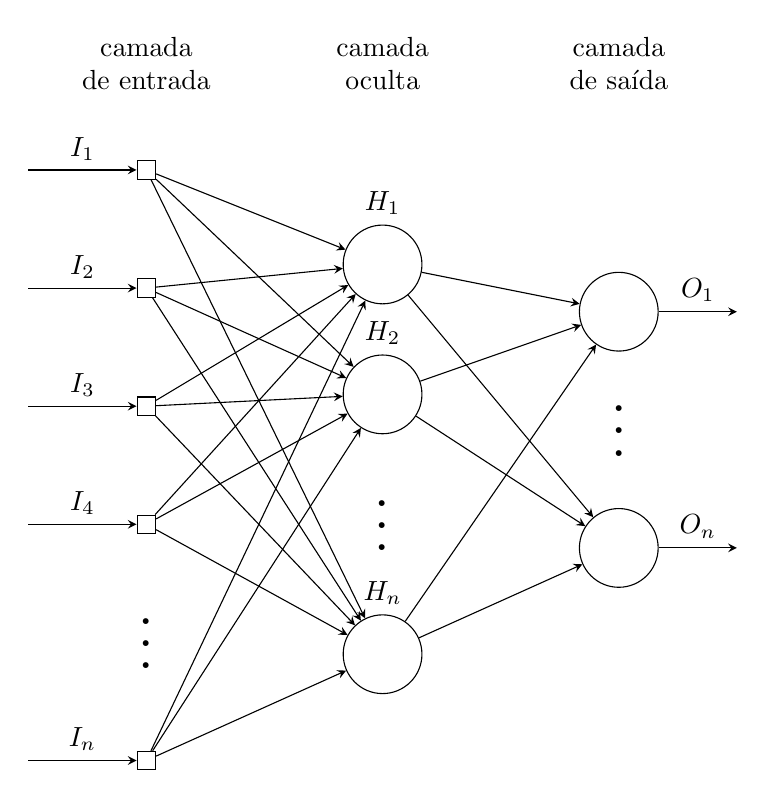
\begin{tikzpicture}[x=1.5cm, y=1.5cm, >=stealth]

\foreach \m/\l [count=\y] in {1,2,3,4,missing,5}
  \node [every input/.try, input \m/.try] (input-\m) at (0,2.7-\y) {};

\foreach \m [count=\y] in {1,2,missing,3}
  \node [every neuron/.try, neuron \m/.try ] (hidden-\m) at (2,2-\y*1.1) {};

\foreach \m [count=\y] in {1,missing,2}
  \node [every neuron/.try, neuron \m/.try ] (output-\m) at (4,1.5-\y) {};

\foreach \l [count=\i] in {1,2,3,4,n}
  \draw [<-] (input-\i) -- ++(-1,0)
    node [above, midway] {$I_\l$};

\foreach \l [count=\i] in {1,2,n}
  \node [above] at (hidden-\i.north) {$H_\l$};

\foreach \l [count=\i] in {1,n}
  \draw [->] (output-\i) -- ++(1,0)
    node [above, midway] {$O_\l$};

\foreach \i in {1,...,5}
  \foreach \j in {1,...,3}
    \draw [->] (input-\i) -- (hidden-\j);

\foreach \i in {1,...,3}
  \foreach \j in {1,...,2}
    \draw [->] (hidden-\i) -- (output-\j);

\foreach \l [count=\x from 0] in {de entrada, oculta, de sa\'ida}
  \node [align=center, above] at (\x*2,2.3) {camada \\ \l};

\end{tikzpicture}
		\caption{Diagrama de ANN generica}
	\end{centering}	
\end{figure}
\subsection{SCG}
teoria e como funciona
\section{Redes Neurais}
\begin{figure}[!htp]
	\begin{centering}
		%\tikzstyle{block} = [
		% The shape:
		rectangle split,
		rectangle split parts =1,
		% The size:
		minimum size=6mm,
		draw,
		text badly centered,
		draw=blue!80!black!40,
		text=black,
	]
\tikzstyle{decision} = [
		diamond,
		draw,
		text badly centered,
		color=blue,
		aspect=2,
		inner sep=1.5pt,
]
\tikzstyle{begin} = [
		rounded rectangle,
		draw,
		text badly centered,
		minimum size = 1cm,
		color=blue,
]
\tikzstyle{coord} = [
-stealth,
inner sep =0 pt,
]
\begin{tikzpicture}[node distance= 0.6cm,
transition/.style={very thick,->}
]

\node [begin] (start) {\textbf{In\'icio}};

\node [block,rectangle split parts=4] (1) [below=of start] 
	 {\nodepart{one} Escolha 
	  \nodepart{two} $\textbf{w}_1$ 
	  \nodepart{three} $0 < \sigma \leq 10^{-4}$
	  \nodepart{four} $0 < \lambda_1  \leq 10^{-6}$
     };

\node [block,rectangle split parts=4] (2) [below=of 1] {
	\nodepart{one} $\textbf{r}_1 = \textbf{r}_1 = E'(\textbf{w}_1) $
	\nodepart{two} $n = 1 $
	\nodepart{three} $ \text{success} = true $
	\nodepart{four} $\overline{\lambda}_1 = 0 $
	};

\node [decision] (3) [below=of 2]{success};

\node [coord] (c1) [right=of 3.east]{};

\node [coord] (c2) [right=of 1.east]{};

\node [block,rectangle split parts = 3] (4) [right=of c2] {
	\nodepart{one} $\sigma _n =\frac{\sigma}{\left| \textbf{p}_n \right| } $
	\nodepart{two} $\textbf{s}_n = \frac{E' ( \textbf{w}_n + \sigma_n \textbf{p}_n) - E' ( \textbf{w}_n )}{ \sigma_n}  $
	\nodepart{three} $\delta_n = \textbf{p}_n \cdot \textbf{s}_n $ 
};

\node [block] (5) [below=of 4] {
	\nodepart{one} $\delta_n =\delta_n + (\lambda_n - \overline{\lambda}_n ) \left| \textbf{p}_n \right| ^2 $
 };

\node [decision] (6) [below=of 5]{ $\delta_n \leq 0 $ };

\node [block,rectangle split parts=3] (7) [below=of 6]{
	\nodepart{one} $ \overline{\lambda}_n = 2 \left( \lambda_n - \frac{\delta_n}{\left| \textbf{p}_n \right| ^2}\right) $ 
	\nodepart{two} $\delta_n = - \delta_n \left| \textbf{p}_n \right| ^2$
	\nodepart{three} $\lambda_n = \overline{\lambda}_n$
};

\node [block, rectangle split parts = 2] (8) [below=of 7]{
	\nodepart{one} $ \mu_n = \textbf{p}_n \cdot \textbf{r}_n $
	\nodepart{two} $ \alpha_n = \frac{\mu_n}{\delta_n}  $
};

\node [block] (9) [below=of 8]{
	\nodepart{one} $\Delta_n = 2 \delta_n \frac{\left[ E(\textbf{w}_n) - E(\textbf{w}_n + \alpha_n \textbf{p}_n) \right]}{\mu_n ^2}$
};

\node [decision] (10) [below=of 9]{
	$\Delta_n \geq 0 $
};


\node [coord] (c3) [right=of 10] {};
\node [coord] (c4) [right=of 4] {};


\node [block,rectangle split parts=4] (11) [right=of c4]{
	\nodepart{one} $\textbf{w}_{n+1} = \textbf{w}_n + \alpha_n \textbf{p}_n$
	\nodepart{two} $\textbf{r}_{n+1} = - E (\textbf{w}_{n+1} )$
	\nodepart{three} $ \overline{\lambda}_n = 0 $
	\nodepart{four} $ success = true $
};

\node [decision] (12) [below=of 11]{$n \text{ mod }N = 0 $};

\node [block](13) [right=of 12]{
	$\textbf{p}_{n+1} = \textbf{r}_{n+1}$
};


\node [coord] (c5) [above=of 11] {};

\node [block, rectangle split parts=2] (14) [below=of 12]{
	\nodepart{one} $\beta_n  =\frac{ \left| \textbf{r}_{n+1}\right|^2 - \textbf{r}_{n} \cdot \textbf{r}_{n+1} }{\mu_n} $
	\nodepart{two} $\textbf{p}_{n+1} = \textbf{r}_{n+1} \beta_n  \textbf{p}_{n} $
};

\node [decision] (15) [below=of 14] {$\Delta_n \geq 0.75 $};

\node [block] (15true) [right=of 15] {$\lambda_n =\frac{1}{4} \lambda_n $};

\node [block,rectangle split parts=2] (16) [below=of 10] {
	\nodepart{one} $\overline{\lambda}_n = \lambda_n $
 	\nodepart{two} $\text{success} = false $
};

\node [decision] (17) [below=of 15] {$ \Delta_n < 0.25$};

\node [block] (17true) [right=of 17] {$\lambda_n = \lambda_n \frac{\delta_k \left( 1- \Delta_n \right) }{\left| \textbf{p}_{n}\right|^2} $ };

\node [decision] (18) [below=of 17] {$ \textbf{r}_n \neq 0 $};

\node [block] (19) [below=of 18] {$ n = n + 1$};

\node [begin] (end) [right=of 19] {\textbf{Fim}};

\node [coord] (c6) [below=of 16]{};

\node [coord] (c7) [left=of 5]{};

%\node [coord] (c8) [right=of 6] {};

\node [coord] (c9) [left=of 7] {};

\draw [transition] (start) -- (1);
\draw [transition] (1) -- (2);
\draw [transition] (2) -- (3);
\draw [transition,color=green] (3.east) -| node [midway,above] {\tiny{\textbf{true}}}  (c1) -| (c2) -- (4.west);
\draw [transition,color=red] (3.south) -| node [midway,below] {\tiny{\textbf{false}}}  (c7) -- (5.west);

\draw [transition] (4) -- (5);
\draw [transition] (5) -- (6);
\draw [transition,color=green] (6) -- node [midway,below,rotate=-90] {\tiny{\textbf{true}}}  (7);
\draw [transition,color=red] (6.west) -| node [midway,above] {\tiny{\textbf{false}}}  (c9) |- (8.west);

\draw [transition] (7) -- (8);
\draw [transition,color=green] (6) -- node [midway,below,rotate=-90] {\tiny{\textbf{true}}}  (7);
\draw [transition] (8) -- (9);
\draw [transition] (9) -- (10);
\draw [transition,color=red] (10) -- node [midway,below,rotate=-90]{\tiny{false}}(16);
\draw [transition,color=green] (10.east) -| node [midway,below] {\textbf{true}}  (c3) -| (c4) |- (11.west);
\draw [transition] (11) -- (12);
\draw [transition,color=green] (12) -- node [midway,below ] {\tiny{\textbf{true}}} (13);
\draw [very thick] (13.north)  edge [ out=90,in = 0,to path={|- (\tikztotarget)}] (c5);
\draw [transition] (c5) -| (4.north);
\draw [transition,color=red] (12) -- node [midway,below,rotate=-90]{\tiny{false}}(14);
\draw [transition] (14) -- (15);
\draw [transition,color=green] (15) -- node [midway,below] {\tiny{\textbf{true}}}  (15true);
\draw [transition,color=red] (15) -- node [midway,below,rotate=-90]{\tiny{false}}(17);
\draw [transition] (15true) |- (17.north);
\draw [transition,color=green] (17) -- node [midway,below] {\tiny{\textbf{true}}}  (17true);
\draw [transition,color=red] (17) -- node [midway,below,rotate=-90]{\tiny{false}}(18);
\draw [transition] (17true) |- (18.north);
\draw [transition,color=red] (18) -- node [midway,below,rotate=-90]{\tiny{false}}(19);
\draw [transition,color=green] (18) -| node [midway,above] {\tiny{\textbf{true}}}  (end);
\draw [transition] (19) |- (c6) -| (3.west);
\end{tikzpicture}
		\caption{Diagramma SCG}
	\end{centering}	
\end{figure}
\subsection{SCG}
 \cite{MollerSCG}
\section{Support Vector Machine}

teoria e como funciona \cite{Vapnik95} \cite{SVM2017}




Artigos e trabalhos que incentivaram ao TCC.
